\newpage
\subsubsection{Sensor Setup and Calibration}
\hfill
\\
\indent An understanding of how the sensors operate is required before they can be correctly integrated into the system.  
This involves studying their configuration tools, calibration procedures, and data output formats.  
Only by understanding their internal operation and limitations can they be properly adapted for the precise requirements of this application.

\vspace{0.5em}
\noindent\textbf{Radar Setup and Calibration}
\label{sec:radar_setup_calibration}
\vspace{0.5em}

\paragraph{Configuration Tools}
\hfill
\\
\indent To configure and validate the radar sensors, two official Texas Instruments tools were employed: the \textit{mmWave Demo Visualizer} and the \textit{mmWave Sensing Estimator}.  
These tools allowed the rapid prototyping of chirp profiles and provided immediate feedback on their impact on range and velocity performance.  

The \textbf{mmWave Demo Visualizer} \cite{mmwave_demo_web, mmwave_demo_doc} is a browser-based application that enables basic sensor configuration and visualization.  
It allows the user to adjust frame rate, range resolution, maximum range, and velocity settings, while simultaneously observing output plots such as point clouds, noise profile, range profile, and Doppler heatmaps.  
This tool was particularly useful for testing standard chirp configurations and ensuring the correct operation of the radar hardware in a controlled environment.  
Figure~\ref{fig:mmwave_demo_visualizer} shows an example of the configuration interface.  

\begin{figure}[!htbp]
    \centering
    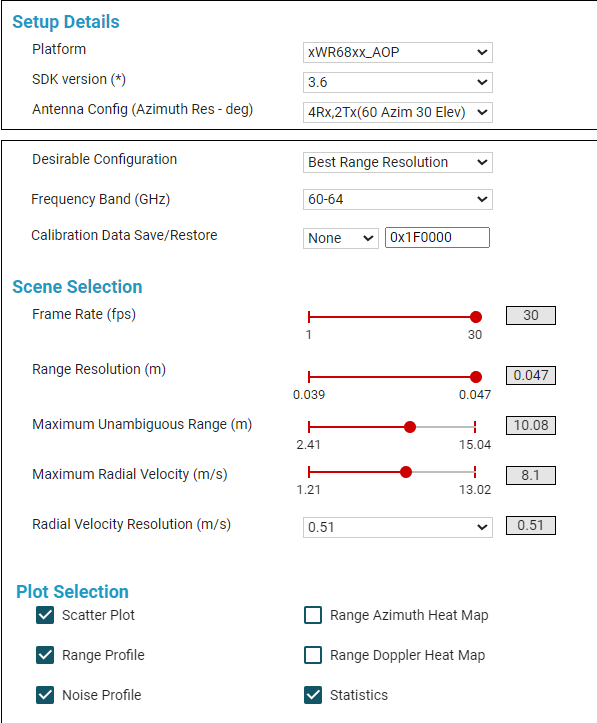
\includegraphics[width=0.9\linewidth]{images/mmWaveDemoVisualizer.png}
    \caption{mmWave Demo Visualizer interface for radar setup and visualization.\\
    \textit{Source: Texas Instruments, available at \href{https://dev.ti.com/gallery/view/mmwave/mmWave_Demo_Visualizer/ver/3.6.0/}{dev.ti.com}}}
    \label{fig:mmwave_demo_visualizer}
\end{figure}

Complementing this, the \textbf{mmWave Sensing Estimator} \cite{mmwave_demo_output} provides a theoretical framework to design chirp profiles.  
By specifying parameters such as slope, bandwidth, ADC sampling rate, and frame timing, the tool outputs derived radar capabilities including range resolution, maximum detectable velocity, and unambiguous range.  
However, it must be emphasized that the estimator only generates feasible profiles. However, it does not guarantee hardware compatibility.  
Each configuration must be tested on the actual radar device to confirm correct execution.  
Figure~\ref{fig:mmwave_sensing_estimator} illustrates the chirp design interface of the estimator.  

\begin{figure}[!htbp]
    \centering
    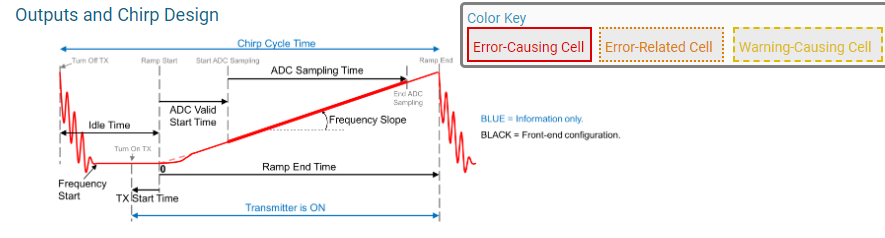
\includegraphics[width=0.9\linewidth]{images/sensingEstimatorChirp.png}
    \caption{mmWave Sensing Estimator interface for chirp configuration design.\\
    \textit{Source: Texas Instruments, available at \href{https://dev.ti.com/gallery/view/mmwave/mmWaveSensingEstimator/ver/2.5.1/}{dev.ti.com}}}
    \label{fig:mmwave_sensing_estimator}
\end{figure}

\vspace{0.5em}
\paragraph{Chirp Configuration}
\hfill
\\
\indent The IWR6843AOP operates as a Frequency-Modulated Continuous Wave (FMCW) radar, transmitting chirps whose frequency increases linearly over a bandwidth $B$ during a duration $T_c$.  
Reflected signals return with a frequency shift that encodes target range, while Doppler shifts across successive chirps provide relative velocity.  

The chirp is defined by:
\begin{itemize}
    \item Start frequency $f_0$ [GHz]
    \item Frequency slope $S$ [MHz/$\mu$s]
    \item Chirp duration $T_c$ [$\mu$s]
    \item Idle time between chirps $T_{\text{idle}}$ [$\mu$s]
    \item Sampling rate $f_s$ [Msps]
    \item Bandwidth $B = S \cdot T_c$ [MHz]
\end{itemize}
From these parameters, the sensing performance is determined as:
\[
    \Delta R = \frac{c}{2B} \ [\text{m}], \qquad
    R_{\max} = \frac{c f_s}{2S} \ [\text{m}],
\]
\[
    \Delta v = \frac{\lambda}{2 N_c T_c} \ [\text{m/s}], \qquad
    v_{\max} = \frac{\lambda}{4 T_c} \ [\text{m/s}],
\]
where $\Delta R$ is \textbf{range resolution}, $R_{\max}$ the \textbf{maximum unambiguous range}, $\Delta v$ the \textbf{velocity resolution}, and $v_{\max}$ the \textbf{maximum unambiguous velocity}.  

\textbf{Full-Bandwidth Chirp (Single 4 GHz Sweep)}, shown in Fig.~\ref{fig:profile4GHz}, provides the finest possible range resolution by sweeping the entire 4~GHz spectrum in a single chirp.  
This configuration is well suited for precise spatial localization but requires high ADC sampling rates and is more prone to interference, making it practical mainly for single-radar setups.  

\begin{figure}[!htbp]
    \centering
    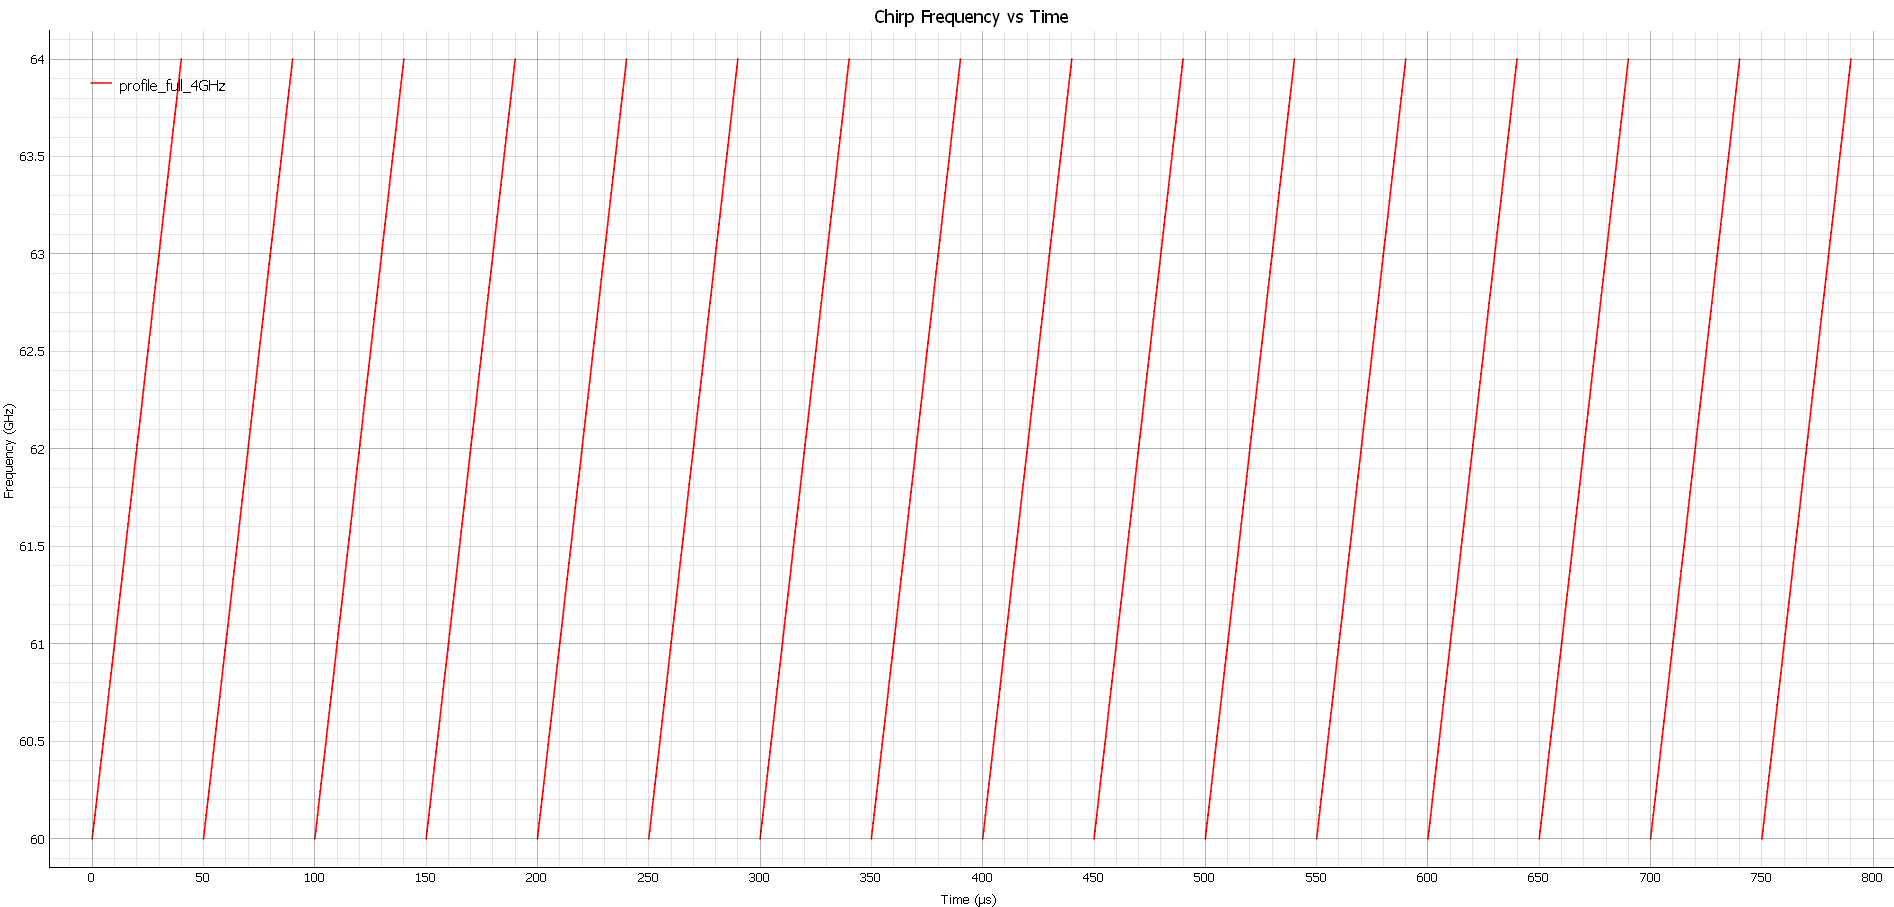
\includegraphics[width=0.7\linewidth]{images/profile_full_4GHz.png}
    \caption{Full-bandwidth chirp (single 4~GHz sweep).  
    \textit{Source: Texas Instruments, available in mmWave Demo Visualizer \cite{mmwave_demo_doc}}}
    \label{fig:profile4GHz}
\end{figure}

\textbf{Divided-Bandwidth Chirps (Two 2~GHz Sweeps)}, shown in Fig.~\ref{fig:profile2GHz}, split the 4~GHz spectrum into two 2~GHz chirps.  
Although this reduces range resolution compared to a full-band sweep, it lowers ADC requirements and enables reliable operation of dual-radar systems.  

In this setup, one chirp configuration was assigned to each radar (Config~A $\rightarrow$ Radar~A, Config~B $\rightarrow$ Radar~B).  
By operating on distinct frequency ranges, the radars avoided spectral overlap, preventing ghost targets and preserving point cloud quality.  

\begin{figure}[!htbp]
    \centering
    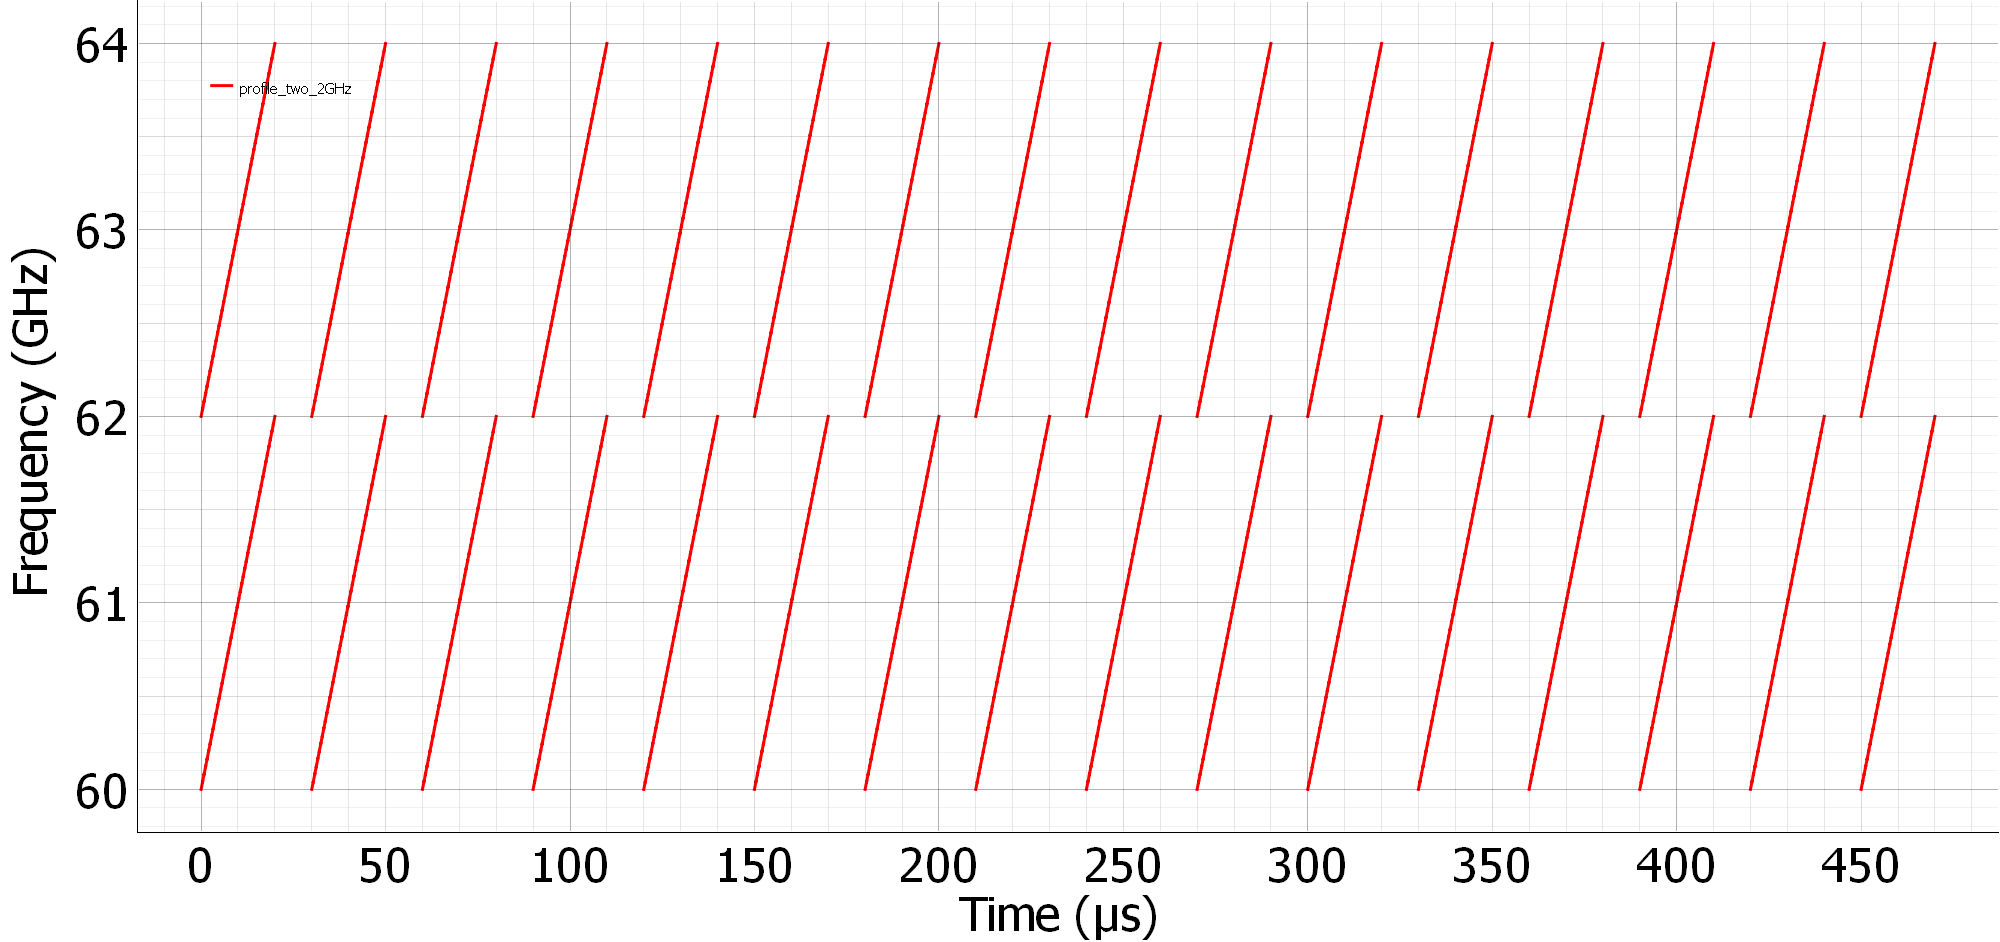
\includegraphics[width=0.7\linewidth]{images/profile_two_2GHz.png}
    \caption{Divided-band chirps (two 2~GHz sweeps).  
    \textit{Source: Texas Instruments, available in mmWave Demo Visualizer \cite{mmwave_demo_doc}}}
    \label{fig:profile2GHz}
\end{figure}

The final parameters were derived using the \textit{mmWave Sensing Estimator} tool \cite{mmwave_demo_output}.  
The divided-band strategy provided a balanced trade-off between resolution and robustness, ensuring stable dual-radar operation while avoiding the interference issues inherent to full-bandwidth sweeps.

\textbf{Same-Band Chirps (Interference Case)} — Using identical chirp configurations on both radars introduced strong mutual interference, which was expected in theory but validated here through practical testing.  
For example, in the vehicle-pushing test (Fig.~\ref{fig:dual_samechirp_pointcloud}) and in the walking-person case (Fig.~\ref{fig:dual_samechirp_cluster}), detections appeared artificially expanded or distorted compared to what was expected, with a single person spanning nearly \SI{3}{\meter}.  
While this spatial deformation was visible in the point clouds, the RANSAC analysis (Fig.~\ref{fig:dual_samechirp_ransac}) provided clearer evidence of the interference, with estimated radial velocities reaching up to $\pm$\SI{5}{\meter\per\second} despite the slow and controlled motions.  
This underlines that the main strength of the radar lies in the Doppler information extracted from detections, which in this case exposed the interference effects more clearly than the point cloud itself.  

These inconsistencies confirm that cross-talk affects both point cloud density and Doppler-based velocity estimation, making odometry unreliable.  
This experiment demonstrated the necessity of separating chirp frequency bands, leading to the adoption of the divided-bandwidth configuration for stable dual-radar operation.

\begin{figure}[!htbp]
    \centering
    \begin{subfigure}{0.48\linewidth}
        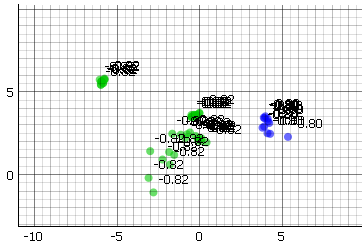
\includegraphics[width=\linewidth]{images/DualSensorSameConfigPointCloud.png}
        \caption{Point cloud of the vehicle-pushing scenario.}
        \label{fig:dual_samechirp_pointcloud}
    \end{subfigure}
    \hfill
    \begin{subfigure}{0.48\linewidth}
        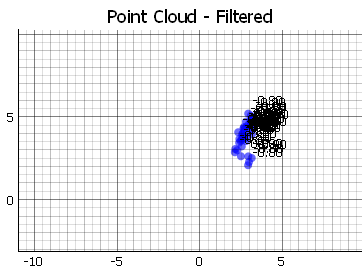
\includegraphics[width=\linewidth]{images/DualSensorSameConfigPointCloudPerson.png}
        \caption{Point cloud of the walking-person scenario.}
        \label{fig:dual_samechirp_cluster}
    \end{subfigure}
    \caption{Point clouds from dual-radar interference with same-band chirps (green = Radar~A, blue = Radar~B).  
    Scenario (a) corresponds to pushing the vehicle, and (b) to a person walking towards the vehicle.}
    \label{fig:dual_samechirp_results}
\end{figure}

\begin{figure}[!htbp]
    \centering
    \begin{subfigure}{0.48\linewidth}
        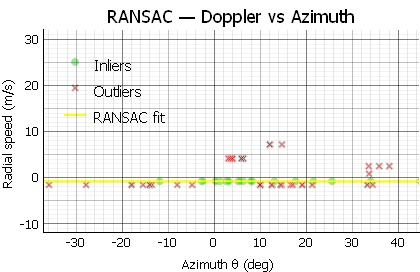
\includegraphics[width=\linewidth]{images/DualSensorSameConfigRansac.png}
        \caption{RANSAC of scenario (a) from Fig.~\ref{fig:dual_samechirp_results}.}
        \label{fig:dual_samechirp_ransac_vehicle}
    \end{subfigure}
    \hfill
    \begin{subfigure}{0.48\linewidth}
        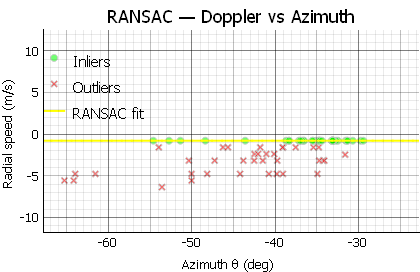
\includegraphics[width=\linewidth]{images/DualSensorSameConfigPersonRansac.png}
        \caption{RANSAC of scenario (b) from Fig.~\ref{fig:dual_samechirp_results}.}
        \label{fig:dual_samechirp_ransac_person}
    \end{subfigure}
    \caption{RANSAC Doppler vs.\ Azimuth for the same-band chirp cases.  
    Both confirm that interference causes incorrect velocity estimates when both radars share the same chirp band.}
    \label{fig:dual_samechirp_ransac}
\end{figure}

\newpage
\noindent\textbf{IMU Setup and Calibration}
\label{sec:imu_setup_calibration}

\setcounter{paragraph}{0} % Restart paragraph numbering

\paragraph{Configuration Tools}
\hfill
\\
The MTi-G-710 was first evaluated with \textit{Xsens MT Manager} to understand the sensor outputs and axis conventions.  
Using the tool, quaternion orientation was visualized in real time while the unit was held still and under gentle rotations to verify stability and drift.  
Reference frames were checked so that the IMU heading and gravity vector aligned with the vehicle-centric frame used in the radar pipeline.  
Output rate, message content, and quaternion format were confirmed in this stage before any integration work.  
This step served only for validation and sanity checks; the final system consumed the IMU stream directly during experiments.  
\vspace{0.5em}
\paragraph{Calibration Aspects}
\hfill
\\
The IMU was mounted on a rigid, nearly horizontal plate at the rear of the vehicle to minimize vibrations and to avoid introducing tilt that would require post-processing.  
On power-up, the device was initialized with a short configuration sequence to enable quaternion output at the desired rate, as specified in the low-level protocol documentation~\cite{mti_lowlevel_doc}.  
This sequence places the device in configuration mode, sets the output configuration (quaternions at a fixed sample rate), and returns it to measurement mode for streaming.  
Because the MTi-G-710 is factory-calibrated and runs an internal sensor-fusion engine, no additional field calibration was required beyond correct mounting and a stable magnetic/metal environment~\cite{mti710_manual}.  
GNSS and velocity outputs were not used in this work; only quaternions were consumed to provide a reliable attitude reference for aligning radar point clouds.  
